\section{挑战-应答:针对主动攻击的安全性}\label{sec:18-6}


现在,我们来考虑一种更强大的攻击,在这种攻击中,对手会主动地冒充合法的验证者。比如说,对手可以克隆一个银行网站,等待用户(即证明者)访问该网站,并与对手一起运行 ID 协议。这样一来,对手就可以反复与用户交互,并向用户发送其选择的任意消息。对手的目标是获得关于验证者密钥 $sk$ 的信息。经过几次这样的交互,对手就转过身来,试图以证明者的身份向合法的验证者发起认证请求。如果对手仍然无法欺骗验证者,我们就称 ID 协议对主动攻击是安全的。

\ref{sec:18-5} 节中介绍的一次性口令协议 \texttt{HOTP} 和 \texttt{Skey} 对主动攻击显然是不安全的。通过冒充验证者,对手能从证明者那里学到新的一次性口令,对手可以用这个口令来向验证者发起认证请求。事实上,只要简单思考,我们就可以发现,没有任何一个单向流协议足以抵御主动攻击。

下面,我们首先给出主动攻击的严格定义,然后构建一个简单的双向流协议,它对主动攻击是安全的。简单起见,在本节中,我们只考虑证明者和验证者都是无状态的协议。

\begin{game}[安全的身份识别:主动攻击]\label{game:18-3}
对于一个给定的身份识别协议 $\mathcal{I}=(G,P,V)$ 和一个给定的对手 $\mathcal{A}$,攻击游戏如图 \ref{fig:18-10} 所示,运行如下:
\begin{itemize}
	\item \emph{密钥生成阶段。}挑战者运行 $(vk,sk)\overset{\rm R}\leftarrow G()$,然后将 $vk$ 发送给对手 $\mathcal{A}$。
	\item \emph{主动探测阶段。}对手请求与证明者进行交互。挑战者与对手在 ID 协议中交互,它扮演证明者的角色,运行算法 $P$,该算法以 $sk$ 初始化。对手扮演验证者的角色,但它不一定遵循验证者的算法 $V$。对手可以与证明者的许多实例并行交互,这些交互可以任意地相互交错进行。
	\item \emph{冒充尝试。}如攻击游戏 \ref{game:18-1} 中一样,挑战者与 $\mathcal{A}$ 交互。挑战者遵循验证者的算法 $V$(以 $vk$ 为输入),而对手 $\mathcal{A}$ 会扮演证明者的角色,但不一定会遵循证明者的算法 $P$。
\end{itemize}
如果验证协议 $V$ 在交互结束时输出 $\mathsf{accept}$,我们就称对手 $\mathcal{A}$ 赢得了游戏。我们将 $\mathcal{A}$ 就 $\mathcal{I}$ 的优势定义为 $\mathrm{ID3}\mathsf{adv}[\mathcal{A}, \mathcal{I}]$,即 $\mathcal{A}$ 赢得游戏的概率。
\end{game}

\begin{figure}
  \centering
  \tikzset{every picture/.style={line width=0.75pt}}

\begin{tikzpicture}[x=0.75pt,y=0.75pt,yscale=-1,xscale=1]

\draw  [fill={rgb, 255:red, 255; green, 255; blue, 255 }  ,fill opacity=1 ][line width=1.2] [general shadow={fill=black,shadow xshift=2.25pt,shadow yshift=-2.25pt}] (5,30) -- (115,30) -- (115,250) -- (5,250) -- cycle ;
\draw  [fill={rgb, 255:red, 255; green, 255; blue, 255 }  ,fill opacity=1 ][line width=1.2] [general shadow={fill=black,shadow xshift=2.25pt,shadow yshift=-2.25pt}] (340,30) -- (450,30) -- (450,250) -- (340,250) -- cycle ;

\draw   (25,200) -- (95,200) -- (95,240) -- (25,240) -- cycle ;
\draw   (25,80) -- (95,80) -- (95,120) -- (25,120) -- cycle ;
\draw   (25,140) -- (95,140) -- (95,180) -- (25,180) -- cycle ;

\draw  [->]  (115,60) -- (338,60) ;

\draw  [<-]  (97,87) -- (340,87) ;
\draw  [->]  (95,113) -- (338,113) ;

\draw  [<-]  (97,147) -- (340,147) ;
\draw  [->]  (95,173) -- (338,173) ;

\draw  [<-]  (97,207) -- (340,207) ;
\draw  [->]  (95,233) -- (338,233) ;

\draw  [->]  (60,240) -- (60,290) ;

\draw (60,15) node   [align=left] {挑战者};
\draw (60,50) node    {$(vk,sk)\overset{\mathrm{R}}{\leftarrow}G()$};
\draw (60,220) node    {$V(vk)$};
\draw (225,56.6) node [anchor=south] [inner sep=0.75pt]    {$vk$};
\draw (395,15) node   [align=left] {对手 $\mathcal{A}$};
\draw (65,287) node [anchor=west] [inner sep=0.75pt] [align=left] {$\mathsf{accept}$ 或 $\mathsf{reject}$};
\draw (225,128) node    {$\vdots$};
\draw (60,100) node    {$P(sk)$};
\draw (60,160) node    {$P(sk)$};

\draw (225,100) node  [align=left] {探测 \#$1$};
\draw (225,160) node  [align=left] {探测 \#$Q$};
\draw (225,220) node  [align=left] {冒充尝试};

\end{tikzpicture}
  \caption{攻击游戏 \ref{game:18-3} 中主动攻击的例子}
  \label{fig:18-10}
\end{figure}

\begin{definition}\label{def:18-8}
如果对于所有的有效对手 $\mathcal{A}$,$\mathrm{ID3}\mathsf{adv}[\mathcal{A}, \mathcal{I}]$ 的值都可忽略不计,我们就称身份识别协议 $\mathcal{I}$ \textbf{对主动攻击是安全的(secure against active attacks)}。
\end{definition}

\begin{snote}[并行攻击 vs. 串行攻击。]
请注意,在攻击游戏的主动探测阶段,我们允许对手同时与证明者的多个实例交互。我们可以考虑一个较弱的攻击模型,在该模型中,这些交互必须按顺序运行,如图 \ref{fig:18-10} 所示。然而,我们考察的所有协议都能在这种更强的、并行的攻击模型中保持安全性。
\end{snote}

\begin{snote}[保持 $vk$ 的机密性。]
一些满足定义 \ref{def:18-8} 的协议并不要求验证者保有任何秘密。然而,我们将要在本节介绍的一个协议确实要求 $vk$ 是秘密的。这就促成了攻击游戏 \ref{game:18-3} 的一个弱化版本,即挑战者不向对手发送 $vk$。正如 \ref{sec:18-5} 节所述,如果 $vk$ 是保密的,我们就必须允许对手与验证者交互,因为这种交互有可能泄露 $vk$ 的信息。因此,在主动探测阶段,我们允许对手同时与证明者和验证者的多个实例交互。当与一个验证者实例交互时,对手会了解验证者输出的是 $\mathsf{accept}$ 还是 $\mathsf{reject}$。此外,在冒充尝试期间,我们让对手同时与多个验证者交互,如果这些验证者中至少有一个接受,对手就赢得了游戏。

我们令 $\mathrm{wID3}\mathsf{adv}[\mathcal{A},\mathcal{I}]$ 为对手赢得这个较弱版本的攻击游戏 \ref{game:18-3} 的优势。在这种设置下安全的身份识别协议被称为是\textbf{弱安全的(weakly secure)}。
\end{snote}

\begin{definition}\label{def:18-9}
如果对于所有的有效对手 $\mathcal{A}$,$\mathrm{wID3}\mathsf{adv}[\mathcal{A},\mathcal{I}]$ 的值都可忽略不计,我们就称 ID 协议 $\mathcal{I}$ \textbf{对主动攻击是弱安全的(weakly secure against active attacks)}。
\end{definition}

\subsection{挑战-应答协议}\label{subsec:18-6-1}

我们介绍两种(无状态)ID 协议,称为\textbf{挑战-应答(challenge-response)},对主动攻击都是安全的。第一种协议是弱安全的,即验证者必须保密 $vk$。对于第二种协议,即使 $vk$ 被公开,它也是安全的。

令 $\mathcal{I}=(S_\mathrm{mac},V_\mathrm{mac})$ 是一个定义在 $(\mathcal{K},\mathcal{M},\mathcal{T})$ 上的 MAC。挑战-应答协议 $\mathtt{ChalResp}_\mathrm{mac} = (G,P,V)$ 如图 \ref{fig:18-11} 所示,运行如下:
\begin{itemize}
	\item $G$:随机选取一个 $k\overset{\rm R}\leftarrow\mathcal{K}$ 并输出 $sk:=k$ 和 $vk:=k$。
	\item 算法 $P$ 被赋予 $sk$,算法 $V$ 被赋予 $vk$,并按如下方式交互:
	\begin{enumerate}
		\item $V$ 随机选取一个 $c\overset{\rm R}\leftarrow\mathcal{M}$,并将 $c$ 发送给 $P$;
		\item $P$ 计算 $t\overset{\rm R}\leftarrow S_\mathrm{mac}(k,c)$,并将 $t$ 发送给 $V$;
		\item $V$ 输出 $V_\mathrm{mac}(k,c,t)$。
	\end{enumerate}
\end{itemize}
随机数 $c$ 被称为\textbf{挑战 (challenge)},$t$ 被称为\textbf{应答 (response)}。显然,为了保证协议的安全性,$vk$ 必须保密。

\begin{figure}
  \centering
  \tikzset{every picture/.style={line width=0.75pt}}   

\begin{tikzpicture}[x=0.75pt,y=0.75pt,yscale=-1,xscale=1]

\draw  [fill={rgb, 255:red, 255; green, 255; blue, 255 }  ,fill opacity=1 ][line width=1.2] [general shadow={fill=black,shadow xshift=2.25pt,shadow yshift=-2.25pt}] (0,60) -- (60,60) -- (60,150) -- (0,150) -- cycle ;
\draw  [fill={rgb, 255:red, 255; green, 255; blue, 255 }  ,fill opacity=1 ][line width=1.2] [general shadow={fill=black,shadow xshift=2.25pt,shadow yshift=-2.25pt}] (250,60) -- (310,60) -- (310,150) -- (250,150) -- cycle ;

\draw  [->]  (140,20) -- (30,55) ;
\draw  [->]  (170,20) -- (280,55) ;

\draw  [<-]  (64,85) -- (250,85) ;
\draw  [->]  (60,125) -- (249,125) ;

\draw  [->]  (280,150) -- (280,190) ;

\draw (30,75) node   [align=left] {证明者};
\draw (280,75) node   [align=left] {验证者};
\draw (155,5) node    {$k\overset{\rm R}\leftarrow\mathcal{K}$};

\draw (155,72) node    {$c\overset{\rm R}\leftarrow\mathcal{M}$};
\draw (155,112) node    {$t\overset{\rm R}\leftarrow S_\mathrm{mac}(k,c)$};

\draw (280,193) node [anchor=north] [inner sep=0.75pt]   [align=left] {$V_\mathrm{mac}(k,m,t)$};
\draw (83,34.1) node [anchor=south east] [inner sep=0.75pt]    {$k$};
\draw (227,34.1) node [anchor=south west] [inner sep=0.75pt]    {$k$};

\end{tikzpicture}
  \caption{基于 MAC 的挑战-应答身份识别}
  \label{fig:18-11}
\end{figure}

\begin{theorem}\label{theo:18-6}
假设 $\mathcal{I}$ 是一个安全的 MAC 系统,并且消息空间的大小 $|\mathcal{M}|$ 是超多项式的。那么 ID 协议 $\mathtt{ChalResp}_\mathrm{mac}$ 对主动攻击是弱安全的。
\end{theorem}

\begin{proof}[证明简述]
如果 $|\mathcal{M}|$ 是超多项式的,就意味着,在每次冒充尝试中,对手收到它之前(在与证明者的交互中)见过的挑战消息的概率可忽略不计。因此,要么这种小概率事件发生,要么对手(在攻击游戏 \ref{game:6-2} 的意义上)攻破了 MAC 系统。
\end{proof}

\begin{figure}
  \centering
  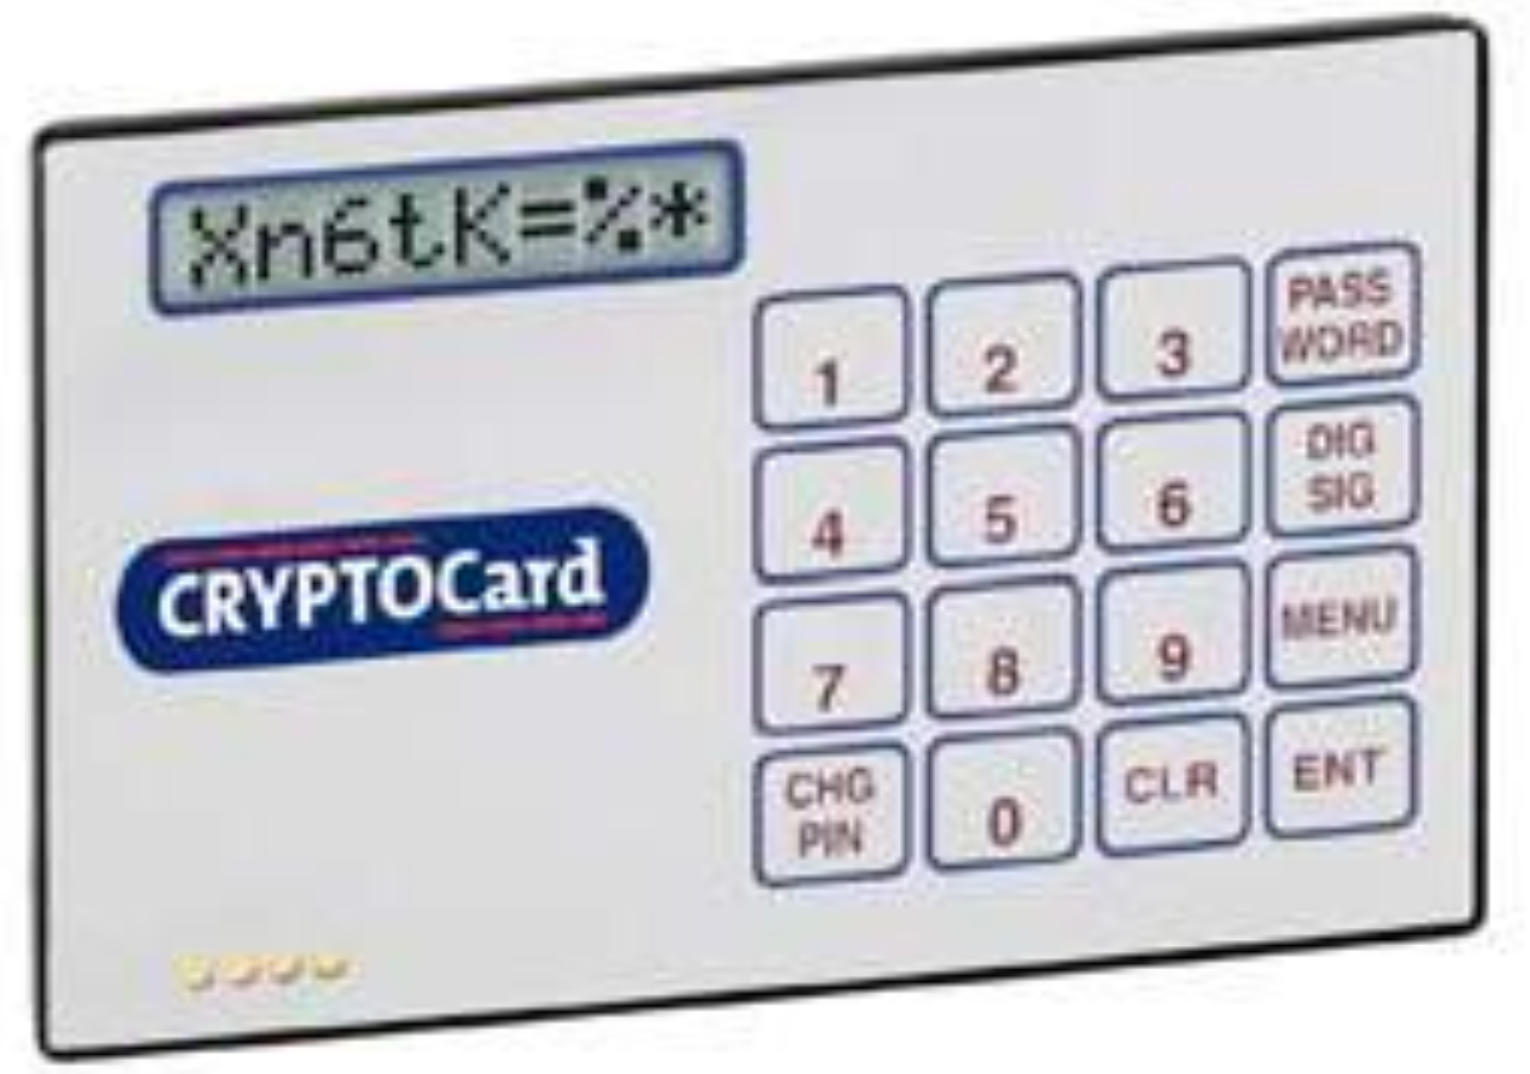
\includegraphics[width=0.25\linewidth]{figures/chapter18/fig12.png}
  \caption{CRYPTOCard RB-1 令牌}
  \label{fig:18-12}
\end{figure}

\begin{snote}[案例研究:CRYPTOCard。]
图 \ref{fig:18-12} 给出了一个挑战-应答令牌的例子。当用户使用他的计算机终端登录到服务器时,服务器会向用户发送一个 $8$ 字符的挑战,该挑战会出现在他的计算机终端屏幕上。用户使用令牌上的小键盘将这个挑战输入令牌。令牌计算出响应,并显示在其屏幕上。然后,用户在他的计算机终端上输入这个响应,并将其发送到服务器,以完成协议。MAC 由一个派生自 3DES 或 AES 的 PRF 实现。
\end{snote}

\begin{snote}[使用口令的挑战-应答。]
在描述协议 $\mathtt{ChalResp}_\mathrm{mac}$ 时,密钥 $k$ 是从底层 MAC 系统的密钥空间 $\mathcal{K}$ 中随机选出的。在某些情况下,部署下面这样的协议是很方便的,它的密钥 $k$ 是由用户生成的口令 $pw$ 推导出来的,比如 $k\leftarrow H(pw)$,其中的 $H$ 是一个 \ref{sec:8-10} 节中介绍的密钥派生函数。

但这可能是相当危险的。如果 $pw$ 是一个弱口令,并且被包含在了某个相对较小的常用密码字典 $\mathcal{D}$ 中,这个协议就很容易受到简单的离线字典攻击。在窃听了证明者和验证者之间单独的某一次对话 $(c,t)$ 后,对手可以进行如下操作:

\vspace*{10pt}

\hspace*{5pt} 对于每个 $w\in\mathcal{D}$:\\
\hspace*{50pt} 如果 $V_\mathrm{mac}\big(H(w),c,t\big)= \mathsf{accept}$:\\
\hspace*{75pt} 输出 $w$ 并停机

\vspace*{10pt}

\noindent
这样,输出的极有可能就是口令 $pw$。
\end{snote}

\subsubsection{使用公开 $vk$ 的挑战应答}\label{subsubsec:18-6-1-1}

图 \ref{fig:18-11} 中的协议很容易转化为 $vk$ 可公开的协议。我们只需用一个定义在 $(\mathcal{M},\mathcal{T})$ 上的签名方案 $(G,S_\mathrm{sig},V_\mathrm{sig})$ 替换 MAC。对 \ref{fig:18-11} 的主要变化是,证明者现在使用算法 $S_\mathrm{sig}$ 和签名私钥来应答挑战。验证者使用算法 $V_\mathrm{sig}$ 和验证公钥来验证应答。我们将所产生协议称为 $\mathtt{ChalResp}_\mathrm{sig}$。

\begin{theorem}\label{theo:18-7}
假设 $\mathcal{S}$ 是一个安全的签名方案,并且消息空间的大小 $|\mathcal{M}|$ 是超多项式的。那么 $\mathtt{ChalResp}_\mathrm{sig}$ 对主动攻击是安全的。
\end{theorem}

\begin{proof}[证明简述]
证明思路与定理 \ref{theo:18-6} 基本相同,只是现在,对手需要伪造的是一个签名,而不是 MAC。
\end{proof}

基于签名的挑战-应答协议拥有明显优于基于 MAC 的挑战-应答协议的安全优势,因为 $vk$ 不需要保密。然而,基于 MAC 的协议的优点在于,它的应答消息可以很短,这对于类似 CRYPTOCard 的应用来说是至关重要的,因为在这种应用中,用户必须在键盘上输入挑战和应答。回顾一下,在 CRYPTOCard 中,应答消息只有 $48$ 比特长。而一个数字签名方案不可能即是安全的,又是短签名的。练习 \ref{exer:18-13} 探讨了另一种挑战-应答协议,在这种协议中,应答消息可以是很短的。